\documentclass[solution,addpoints,12pt]{exam}
\printanswers
\usepackage{amsmath,amssymb}
\usepackage{graphicx}
\newcommand{\RP}{\ensuremath{\mathsf{RP}}}
\newcommand{\expect}[1]{\ensuremath{\mathbb{E}[#1]}}
\newcommand{\dx}{\mathrm{d}x}

\usepackage{graphicx}
\graphicspath{ {./images/} }

\usepackage{hyperref}
\hypersetup{
    colorlinks=true,
    linkcolor=blue,
    filecolor=magenta,      
    urlcolor=cyan,
}
\usepackage{enumitem}
\begin{document}

\hrule
\vspace{3mm}
\noindent 
{\sf IITM-CS6024 : Algorithmic Approaches to Computational Biology  \hfill Date: Oct 23}
\vspace{3mm}\\
\noindent 
{\sf Assignment 5 \hfill Due Date : Oct 27, 23:59}
%{\sf ~\hfill }
\vspace{3mm}
\hrule
\vspace{3mm}
\noindent{{\sf Roll No}:  BE16B002\hfill  {\sf Name}: Anoubhav Agarwaal   }% ROLL NO AND DATE HERE

%{{\sf Collaborators :}}

%{{\sf References:}} %Reference materials, if any.
\vspace{3mm}
\hrule
{\small
\begin{itemize}
    \item Use LaTeX to write-up your solutions, and submit the resulting single pdf file at GradeScope by the due date (Note: As before, {\bf no late submissions} will be allowed, other than one-day late submission with 10\% penalty! Within GradeScope, indicate the page number where your solution to each question starts, else we won't be able to grade it!). 

    \item Collaboration is encouraged, but all write-ups must be done individually and independently, and mention your collaborator(s) if any. %Same rules apply for codes uploaded to HackerRank (i.e., write your own code; we will run plagiarism checks on codes).
    If you have referred a book or any other online material for obtaining a solution, please cite the source. Again don't copy the source {\it as is} - you may use the source to understand the solution, but write-up the solution in your own words. 

  \item This question is less of a standard theory/programming assignment, and more of an investigative practical assignment where you're allowed to use web resources and online tools. The story in this question is fictitious, and any resemblance to actual persons, places or things is purely coincidental.  
\end{itemize}}
\hrule

\begin{questions}
\question
{\bf Prologue:} Having completed a major part of the CS6024 course, you have become a popular sought-after bioinformatician by local health care officials. One morning, you receive a call from an IITM hospital staff that she has collected a viral sample from a patient with grave symptoms and sequence of a gene from that viral sample (which is attached as a sequence in FASTA format in the course moodle). She would like you to use any of the bioinformatics analyses you have learnt in the course to help answer:\\
\\{\bf The Questions:}
\begin{parts}
    \part[6] Which exact viral species the sample belongs to, whether outbreaks of the same viral species (possibly a different strain) has happened in other countries, and which other viral species is closest to this viral species? \\
    ({\em Hint:} NCBI BLAST webtool is your friend! Glossary that may help you interpret BLAST results: cds - coding sequence of a gene that codes for a protein; you may also want to know that UMMC refers to a University in Malaysia)
    \begin{solution}
	The viral species belongs to the Nipah henipavirus. Yes, the outbreaks of the same viral species have happened before in Bangladesh and Malaysia. Nipah henipavirus is closely related to the Hendra henipavirus.
    \end{solution}
    
    \part[6] You may find that at least two other countries had the same viral species outbreak in the past - which of these two countries is closer to the IITM outbreak? Support your answer by providing the length of the longest common subsequence between the IITM viral gene and the same gene from the other country.\\
    ({\em Hint:} Use BLAST output from above that reports a local alignment between the query gene's cds and whole genome or cds from another country; EMBOSS suite of sequence extraction/alignment tools could also help), and
    \begin{solution}
	Bangladesh is closer to the IITM outbreak compared to Malaysia. This can be observed by its relative ranking in the list of hits sorted by score. The length of the longest common subsequence can be calculated by using the following formula :\\ length of LCS = length of query sequence $\times$ query cover  $\times$ percent identity.
The length of the query sequence is 1247.\\
The query cover for the same gene from both countries was 100\%. Hence, the entire query sequence was mapped by the target sequences for the viral gene in both countries. Percent identity is the percentage of characters within the covered part of the query that is identical. This is different for the viral genes of both countries. \\
Percent identity for Bangladesh outbreak gene: 96.79\% \\
Percent identity for Malaysia outbreak gene: 90.46\% \\

Thus, the LCS of the target sequence and query sequence is given by:\\
Length of LCS for Bangladesh outbreak  = 1247 $\times$ 100\% $\times$  96.79\% $\approx 1207$\\
Length of LCS for Malaysia outbreak  = 1247 $\times$ 100\% $\times$  90.46\% $\approx 1128$\\

Length of LCS for Bangladesh outbreak gene $>$ Length of LCS for Malaysia outbreak gene. Thus, Bangladesh outbreak is closer.
    \end{solution}
    
    \part[8] What is the phylogenetic relationship between the IITM viral gene and the other countries' genes? Please provide your answer as a phylogenetic tree diagram.\\
    ({\em Hint:} Take top 20 sequences that BLAST outputs, perform multiple alignment of them using MUSCLE or CLUSTALW to get a distance matrix, and then use Neighbor Joining or other algorithms to get the tree; MEGA software conveniently contains both multiple alignment and Neighbor Joining algorithms; other tools like Phylip are also possible).
    \begin{solution}The MEGA software was used to construct the phylogenetic tree diagram. This was done using the top 25 sequences of BLAST output instead of the top 20 as it did not have any sequences of Malaysian origin. \\
The multiple sequence alignment was performed in MEGA using MUSCLE. The default settings were used, which uses a UPGMA clustering method. The phylogenetic tree diagrams were constructed using distance-based methods such as Neighbor-joining and UPGMA. The results are provided below: \\
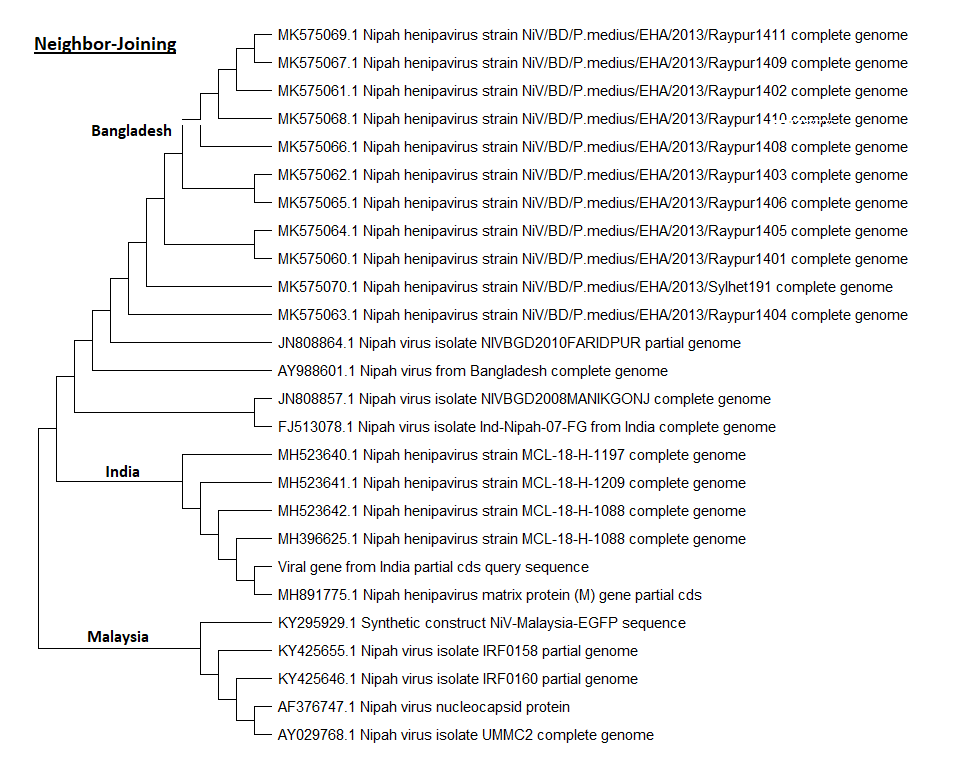
\includegraphics[width=\textwidth]{nj}\vspace{2mm}
From the \textbf{Neighbour-Joining algorithm} tree, \\
We observe that the nodes of the tree that are close to the query sequence are also the ones having high scores in the BLAST report.\\
The \textbf{MCL} strain of the Nipah henipavirus gene originates from India.\\
The \textbf{NiV} strain originates from Bangladesh.\\
The \textbf{UCMMC} Nipah virus isolates originate from Malaysia.\\
We observe that the nodes corresponding to the MCL strain are closer to the query sequence (in the tree) than the NiV strain, and lastly, the UCMMC Nipah virus isolate. This implies that the query sequence has a stronger phylogenetic relationship to the viral genes from India, followed by Bangladesh and, lastly, Malaysia. This matches our observations from our previous analysis.\vspace{2mm} 
\\
From the \textbf{UPGMA algorithm} constructed tree,\\We observe the same phylogenetic relationship, i.e., the query sequence is closer (in the tree) to strains of the Indian viral gene, followed by Bangladesh and last Malaysia. There are a few differences in the terminal branches compared to NJ constructed tree. However, the main branch separation between the three Geographic locations is the same for both trees.\\

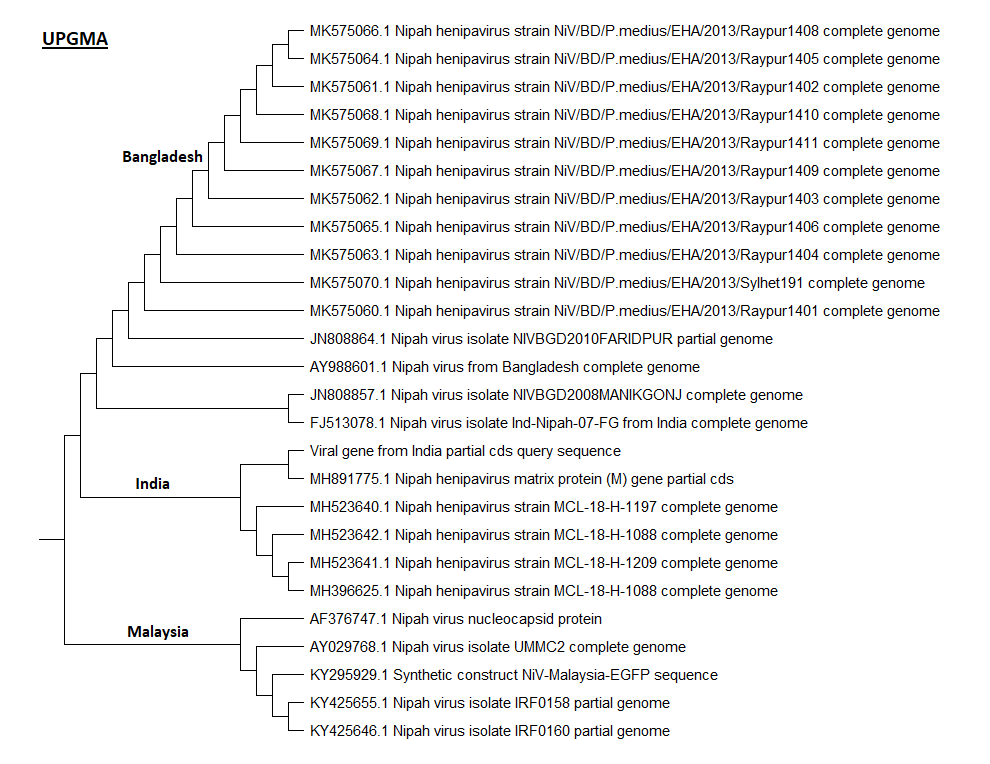
\includegraphics[width=\textwidth]{upgma}
    \end{solution}
    
    \part (bonus 2 points) Which specific research group(s) in the campus or elsewhere in Chennai or Tamil Nadu would you collaborate with to obtain samples from fruit bats and sequence them using Next Generation Sequencing technology to test if fruit bats on the campus could've been the likely carriers of the virus?
    \begin{solution}
	I would collaborate with the Protein Bioinformatics Lab at the Department of Biotechnology at IITM, lead by Prof. M. Michael Gromiha. One of the things they work on is next-generation sequencing analysis. Thus, once the samples (usually urine samples) have been obtained from the fruit bat, the bioinformatics analysis can be performed in collaboration with this research group. However, for collecting samples from fruit bats, I was not able to find any specific research group working on it in Tamil Nadu.\\
This study has already been performed by an international group of scientists in collaboration with the Kerala Agricultural University. Using machine learning, their analysis revealed that at least 11 species of bats in India could be carriers of the Nipah virus. They have published their findings as a research paper.\textsuperscript{\cite{1}}
    \end{solution}
\end{parts}
{\bf Epilogue:} Because patients are waiting for treatment and you have various responsibilities ranging from placements to end-sems to co-curricular activities, you do not have the time to write your own program, and hence are encouraged to use freely available bioinformatics software or online web-resources as indicated in the hints above.

\question[8] Provide an one-page description of the progress your team has made with the course research project. Elaborate on the implementation methods, problems faced, figures generated (e.g., figures you may be trying to reproduce from the paper you are extending), experiments run and results obtained. Also include details on the direction the project is currently taking, benchmarks for experiments you wish to achieve and figures you wish to generate before the final project presentation/report in the week starting Nov 4th.
\begin{solution}
Our primary research objective is to extend the results of Way and Greene(2018)\textsuperscript{\cite{2}} to Deep Variational Auto-Encoders.
The extension will primarily be focused along:
\begin{enumerate}[topsep=0pt]
\itemsep0em 
\item Obtaining a better latent space representation. This is measured by using the encoded features of the latent space for downstream experiments, such as classification.
\item Model interpretability of a Deep VAE using tools like SHAP for obtaining biological insights.
\end{enumerate}
Implementation methods and Figures generated:
\begin{itemize}[topsep=0pt]
\itemsep0em 
\item We have extended the python implementation of the VAE to more number of layers. And have trained the models on a broad set of hyper-parameters such as the number of hidden layers, latent space dimension, warmup, and learning rate. This step required heavy compute resources and was time-consuming.
\item The code for the classification of cancer types, gender, organ type using the above VAE models + classifier has been prepared. We are testing the performance of five or more classifiers on top of the VAE encoded features.
\item The code for t-SNE visualization, hierarchal clustering dendrogram, classification heatmaps have been prepared. We are obtaining a more well-separated t-SNE than the paper.
\item The code for the SHAP library for model interpretation has been explored and implemented.
\end{itemize}
Experiments Run and Results obtained: 
\begin{itemize}[topsep=0pt]
\item We are currently at the cusp of achieving a multitude of results. The bottleneck was training a large number of deep VAE models (having different hyper-parameters), which has been completed. Most of the code files for the downstream experiments (such as pan-cancer classification, t-SNE visualization, obtaining significant genes and pathways, etc.) using these VAE models have been created. Now, we have to run these experiments for all the trained models, collect and analyze the results.
\item One unexpected result while training the VAE models was that the addition of more hidden layers did not improve the reconstruction loss as much as we had expected. However, it was also observed that the latent dimension could be reduced (i.e., higher compression)  from 100 --> 25 dimensions without much difference in reconstruction loss. This was highly interesting as a fixed 100-d latent vector was used in the original paper.
\end{itemize}
The direction of the project and Future targets:
\begin{itemize}[topsep=0pt]
\itemsep0em 
\item We wish to achieve better downstream experiment results using our deep VAE encoded features compared to the shallow VAE in the paper.
\item Most of the computational tasks of the project are soon going to be finished. However, a lot of work has to be done in obtaining biological insights. Hence, the transition from computational tasks to the completion of the biological tasks is the target for the coming week. 
\end{itemize}
\end{solution}

\question[2] Please find below the link to the post-midterm feedback form for the course CS6024. Use your smail ids to access: \url{https://forms.gle/ReSWabMNeVkBGDcH6}. Kindly provide feedback by Assignment deadline. Constructive criticism is encouraged and requested.

\bibliographystyle{ieeetr}
\bibliography{References}
\end{questions}
\end{document}
